\chapter{Result Discussion}
 
  \section{Model building}
  \cite{dondi2008modeling}
  Dondi, Denis, et al. "\textit{Modeling and optimization of a solar energy harvester system for self-powered wireless sensor networks.}" Industrial Electronics, IEEE Transactions on 55.7 (2008): 2759-2766.\\
  
  
  **Initial modelling strategies where based on this paper,  improving the efficiency. \# discrete components\# ** 
 
 
 
 \section{Perturb and Observe Method }
  \begin{figure}[H]
	   \begin{center}
		   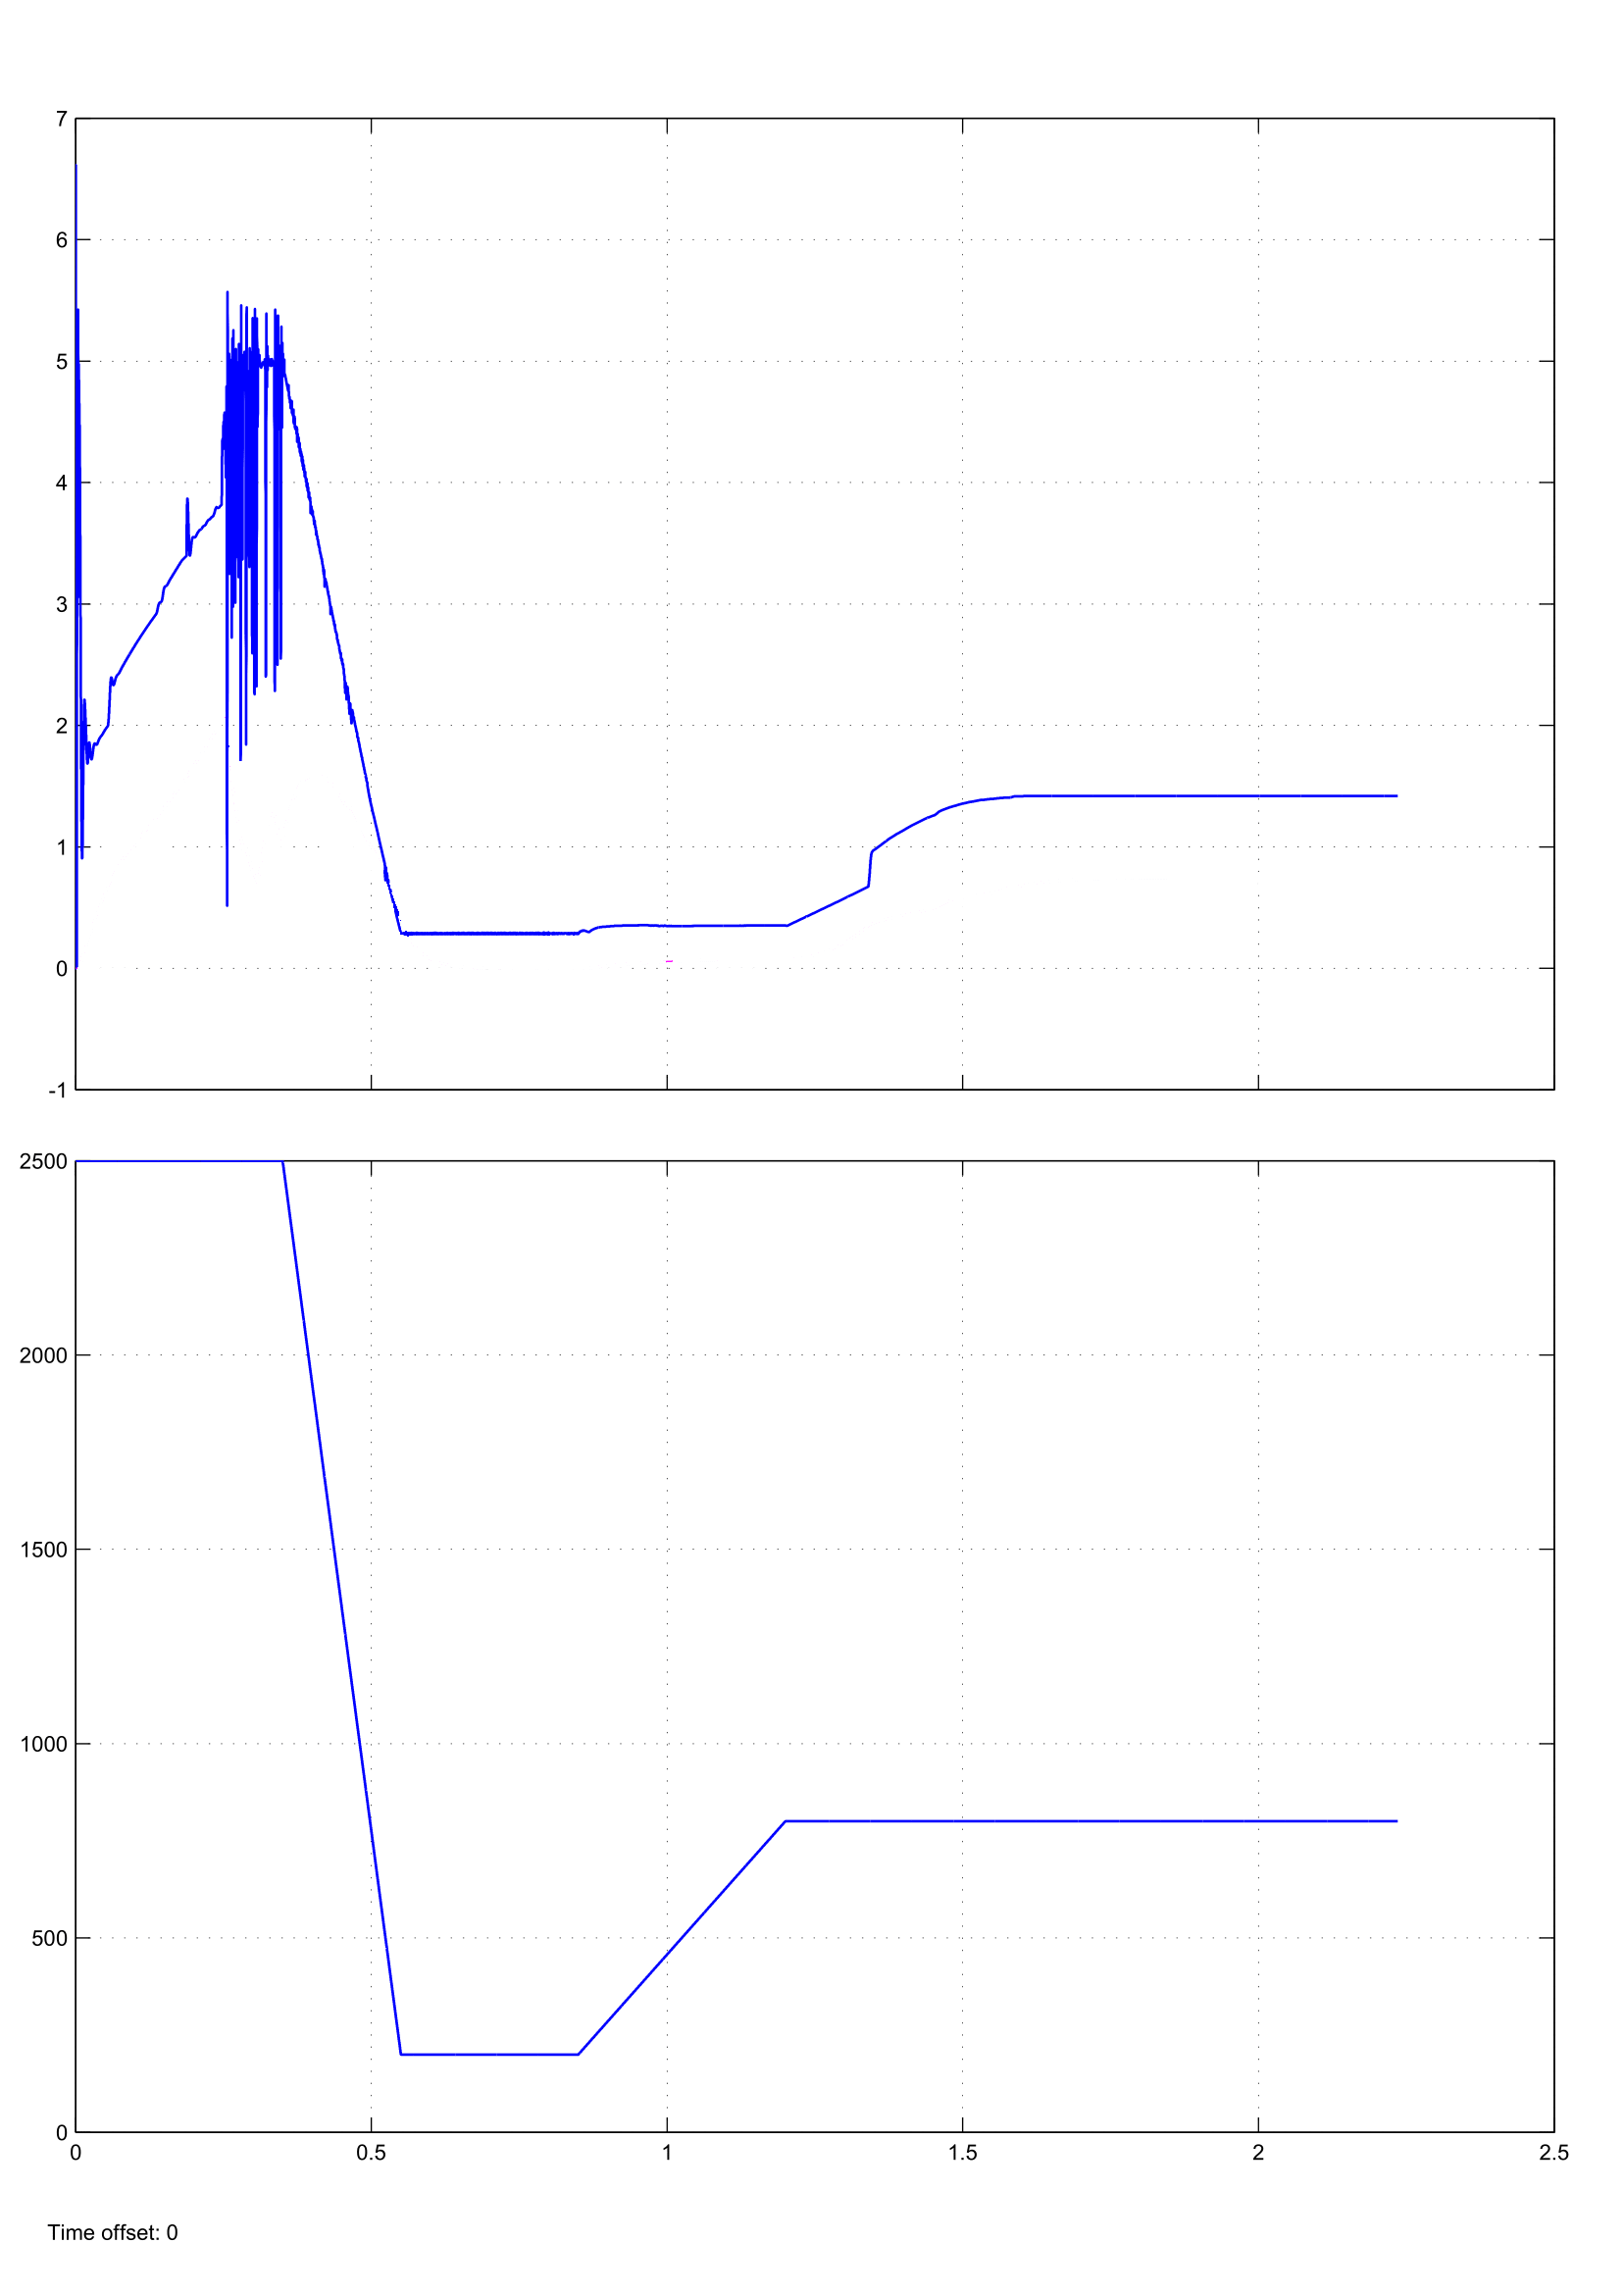
\includegraphics[width=\textwidth]{images/P&O_changing_lux-1}
		   \caption{Perturb and Observe Method on implementation   }
		   \label{fig:PnO_result}
	   \end{center}
   \end{figure}
 \section{Incremental Conductance Method }
 
  \begin{figure}[H]
	   \begin{center}
		   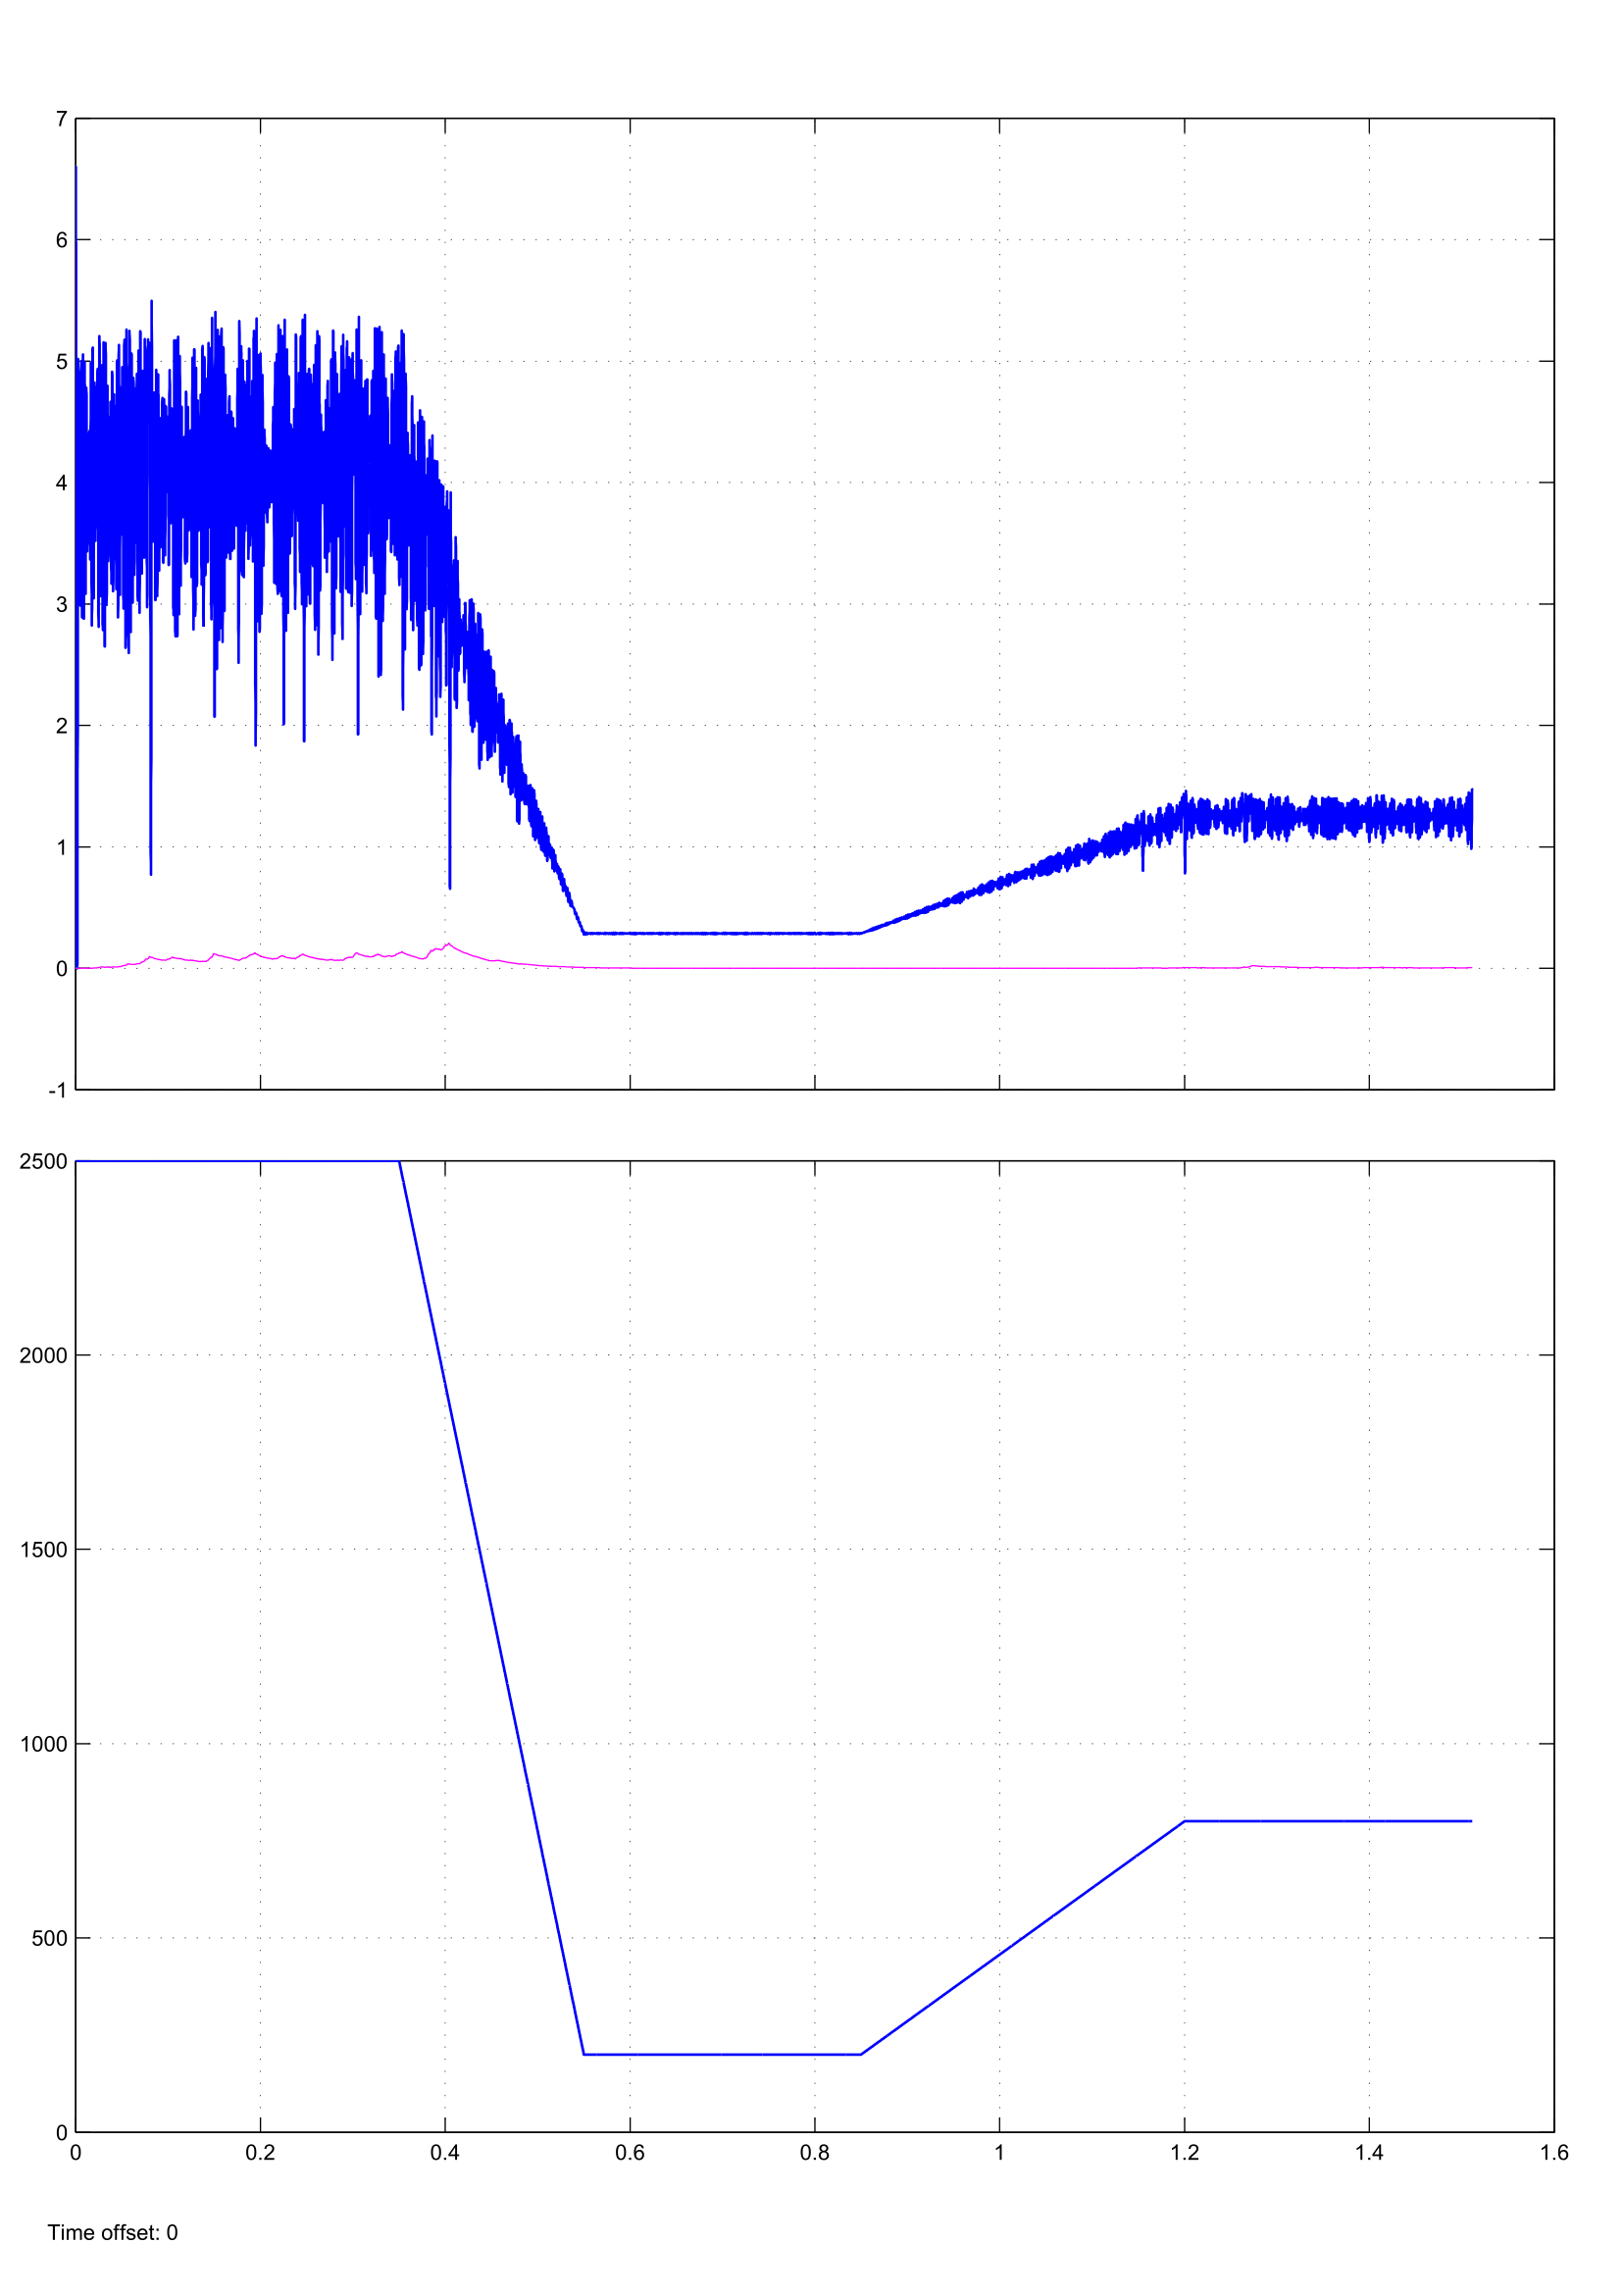
\includegraphics[width=\textwidth]{images/inC_stateflow_changing_lux-1}
		   \caption{Incremental Conductance Method on implementation  }
		   \label{fig:Inc_result}
	   \end{center}
  \end{figure}
 \section{Fractional Open Circuit Voltage Method }
 
 \begin{figure}[H]
	  \begin{center}
		  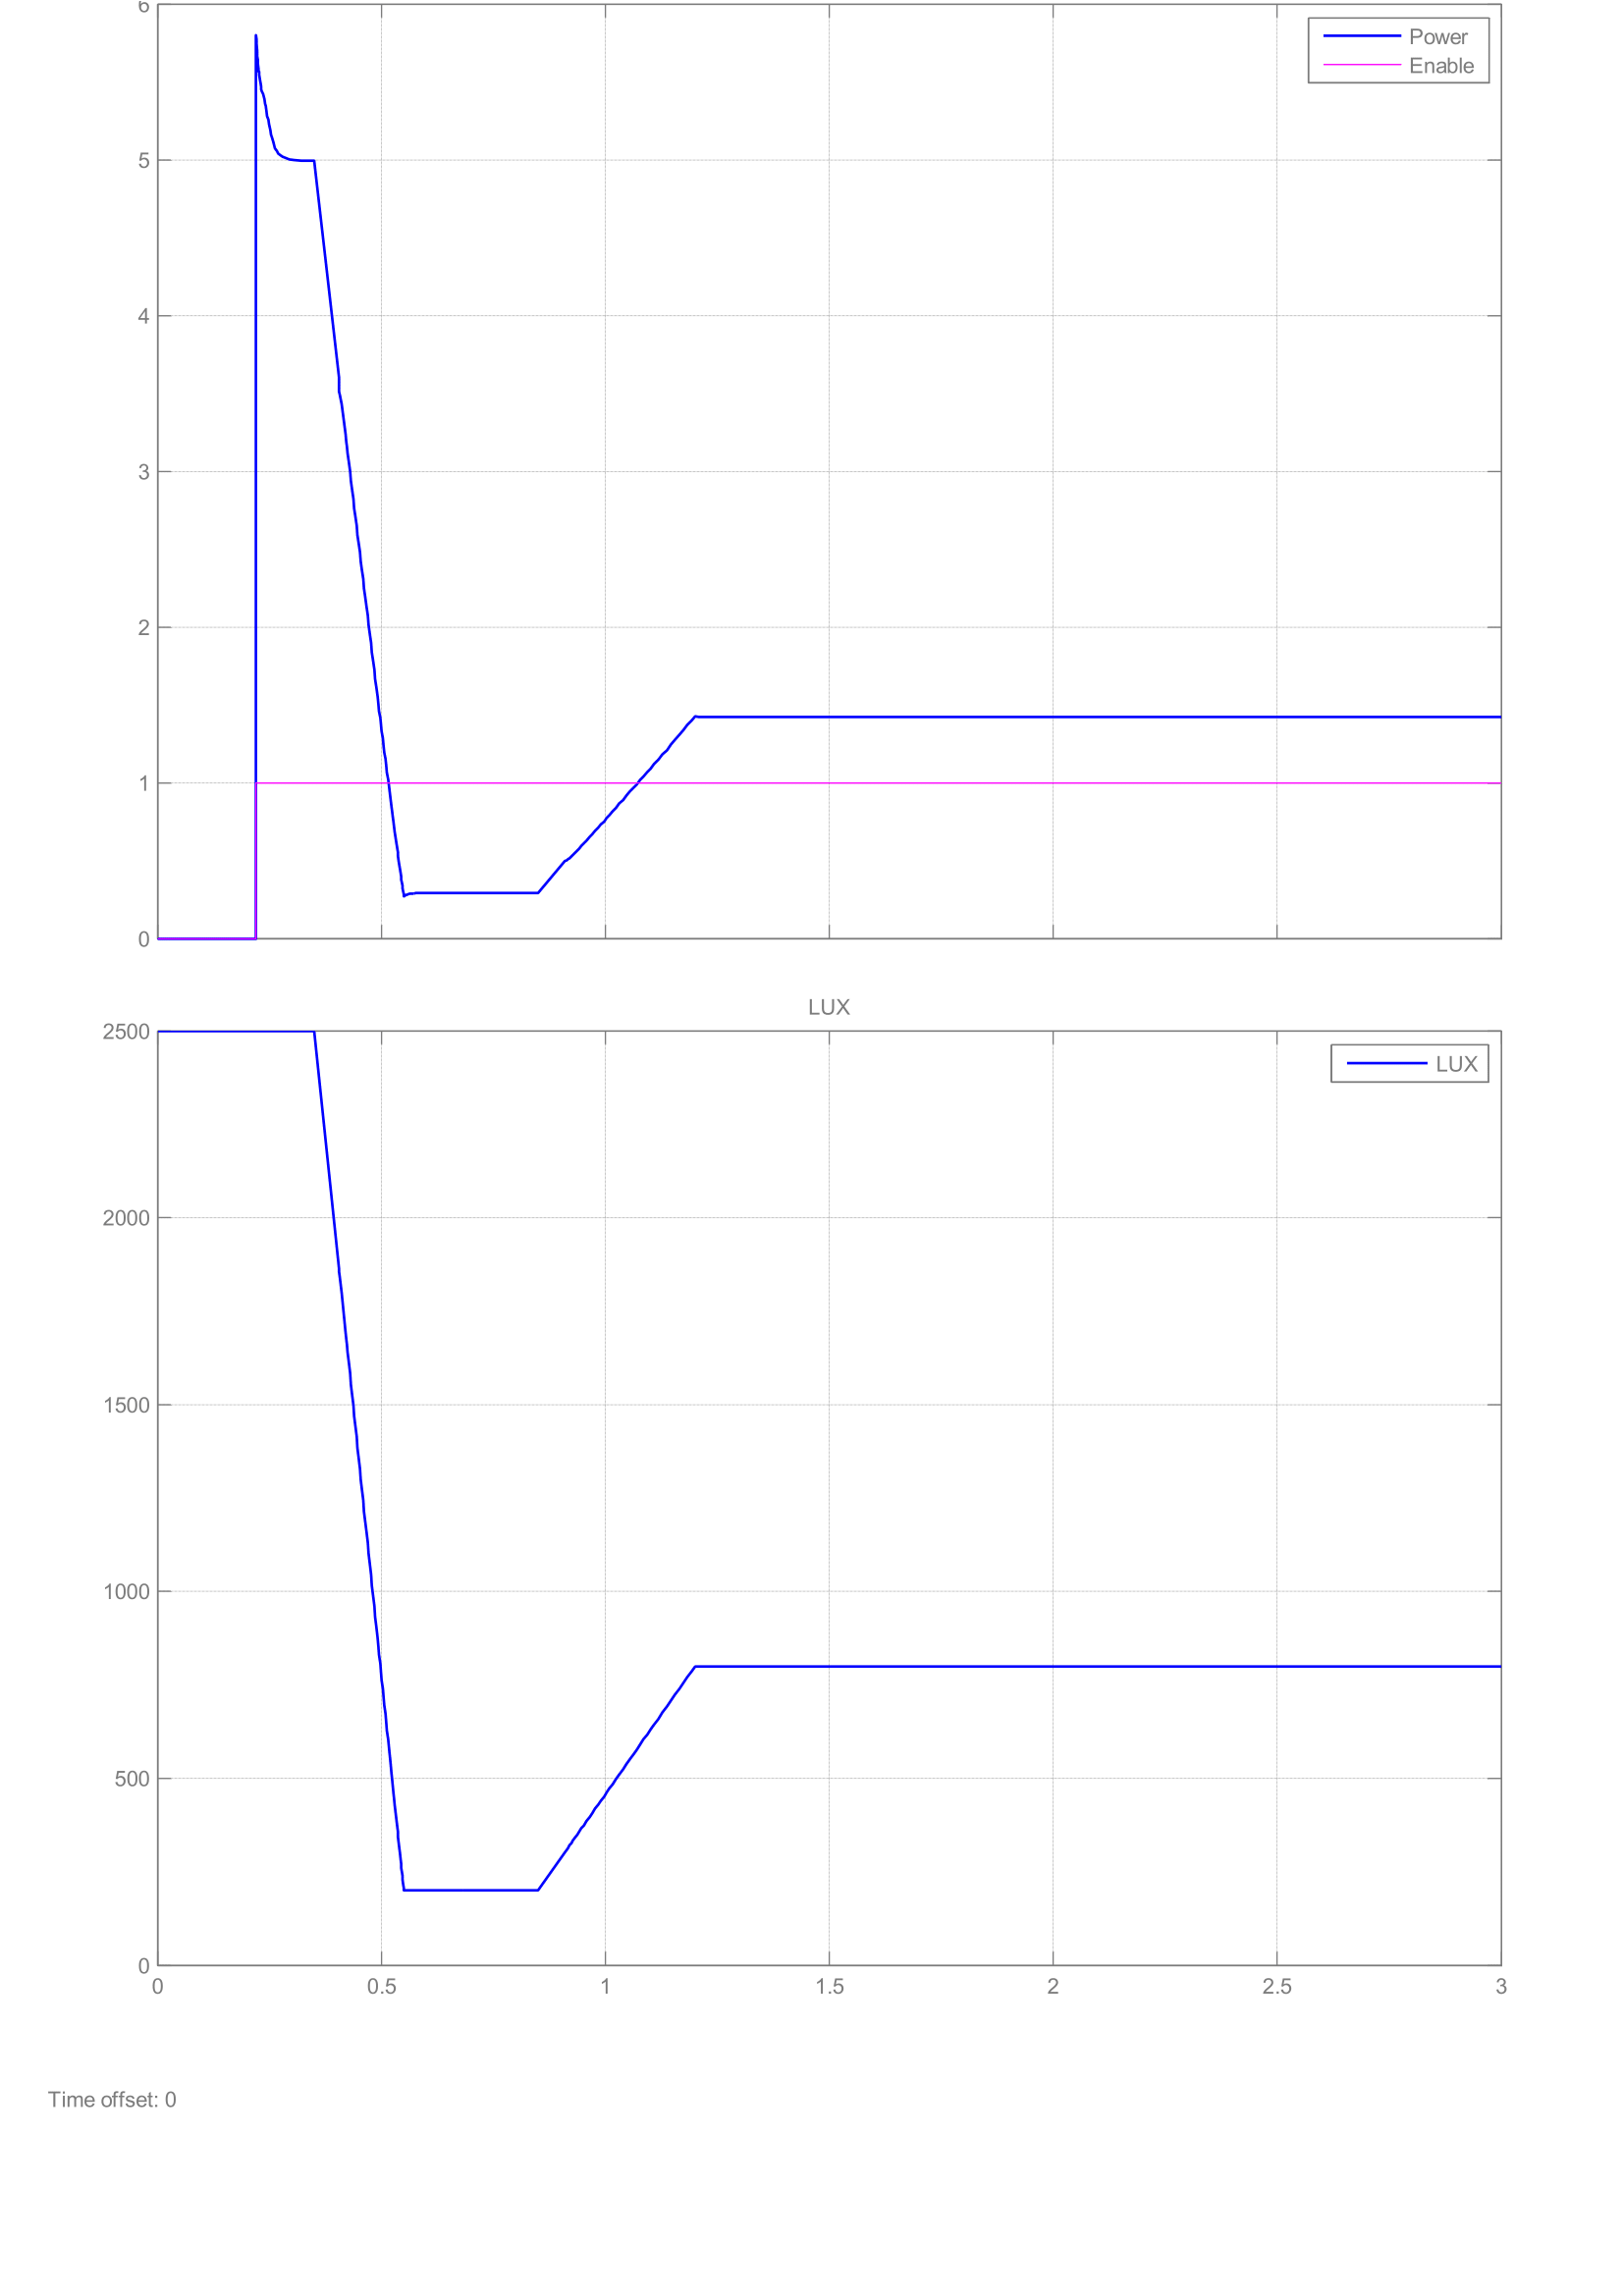
\includegraphics[width=\textwidth]{images/MATLAB_output_test-1}
		  \caption{ Fractional Open Circuit Voltage on implementation}
		  \label{fig:Frac_oc_result}
	  \end{center}
  \end{figure}
\section{Proposed Method }



 \begin{figure}[H]
  \begin{center}
  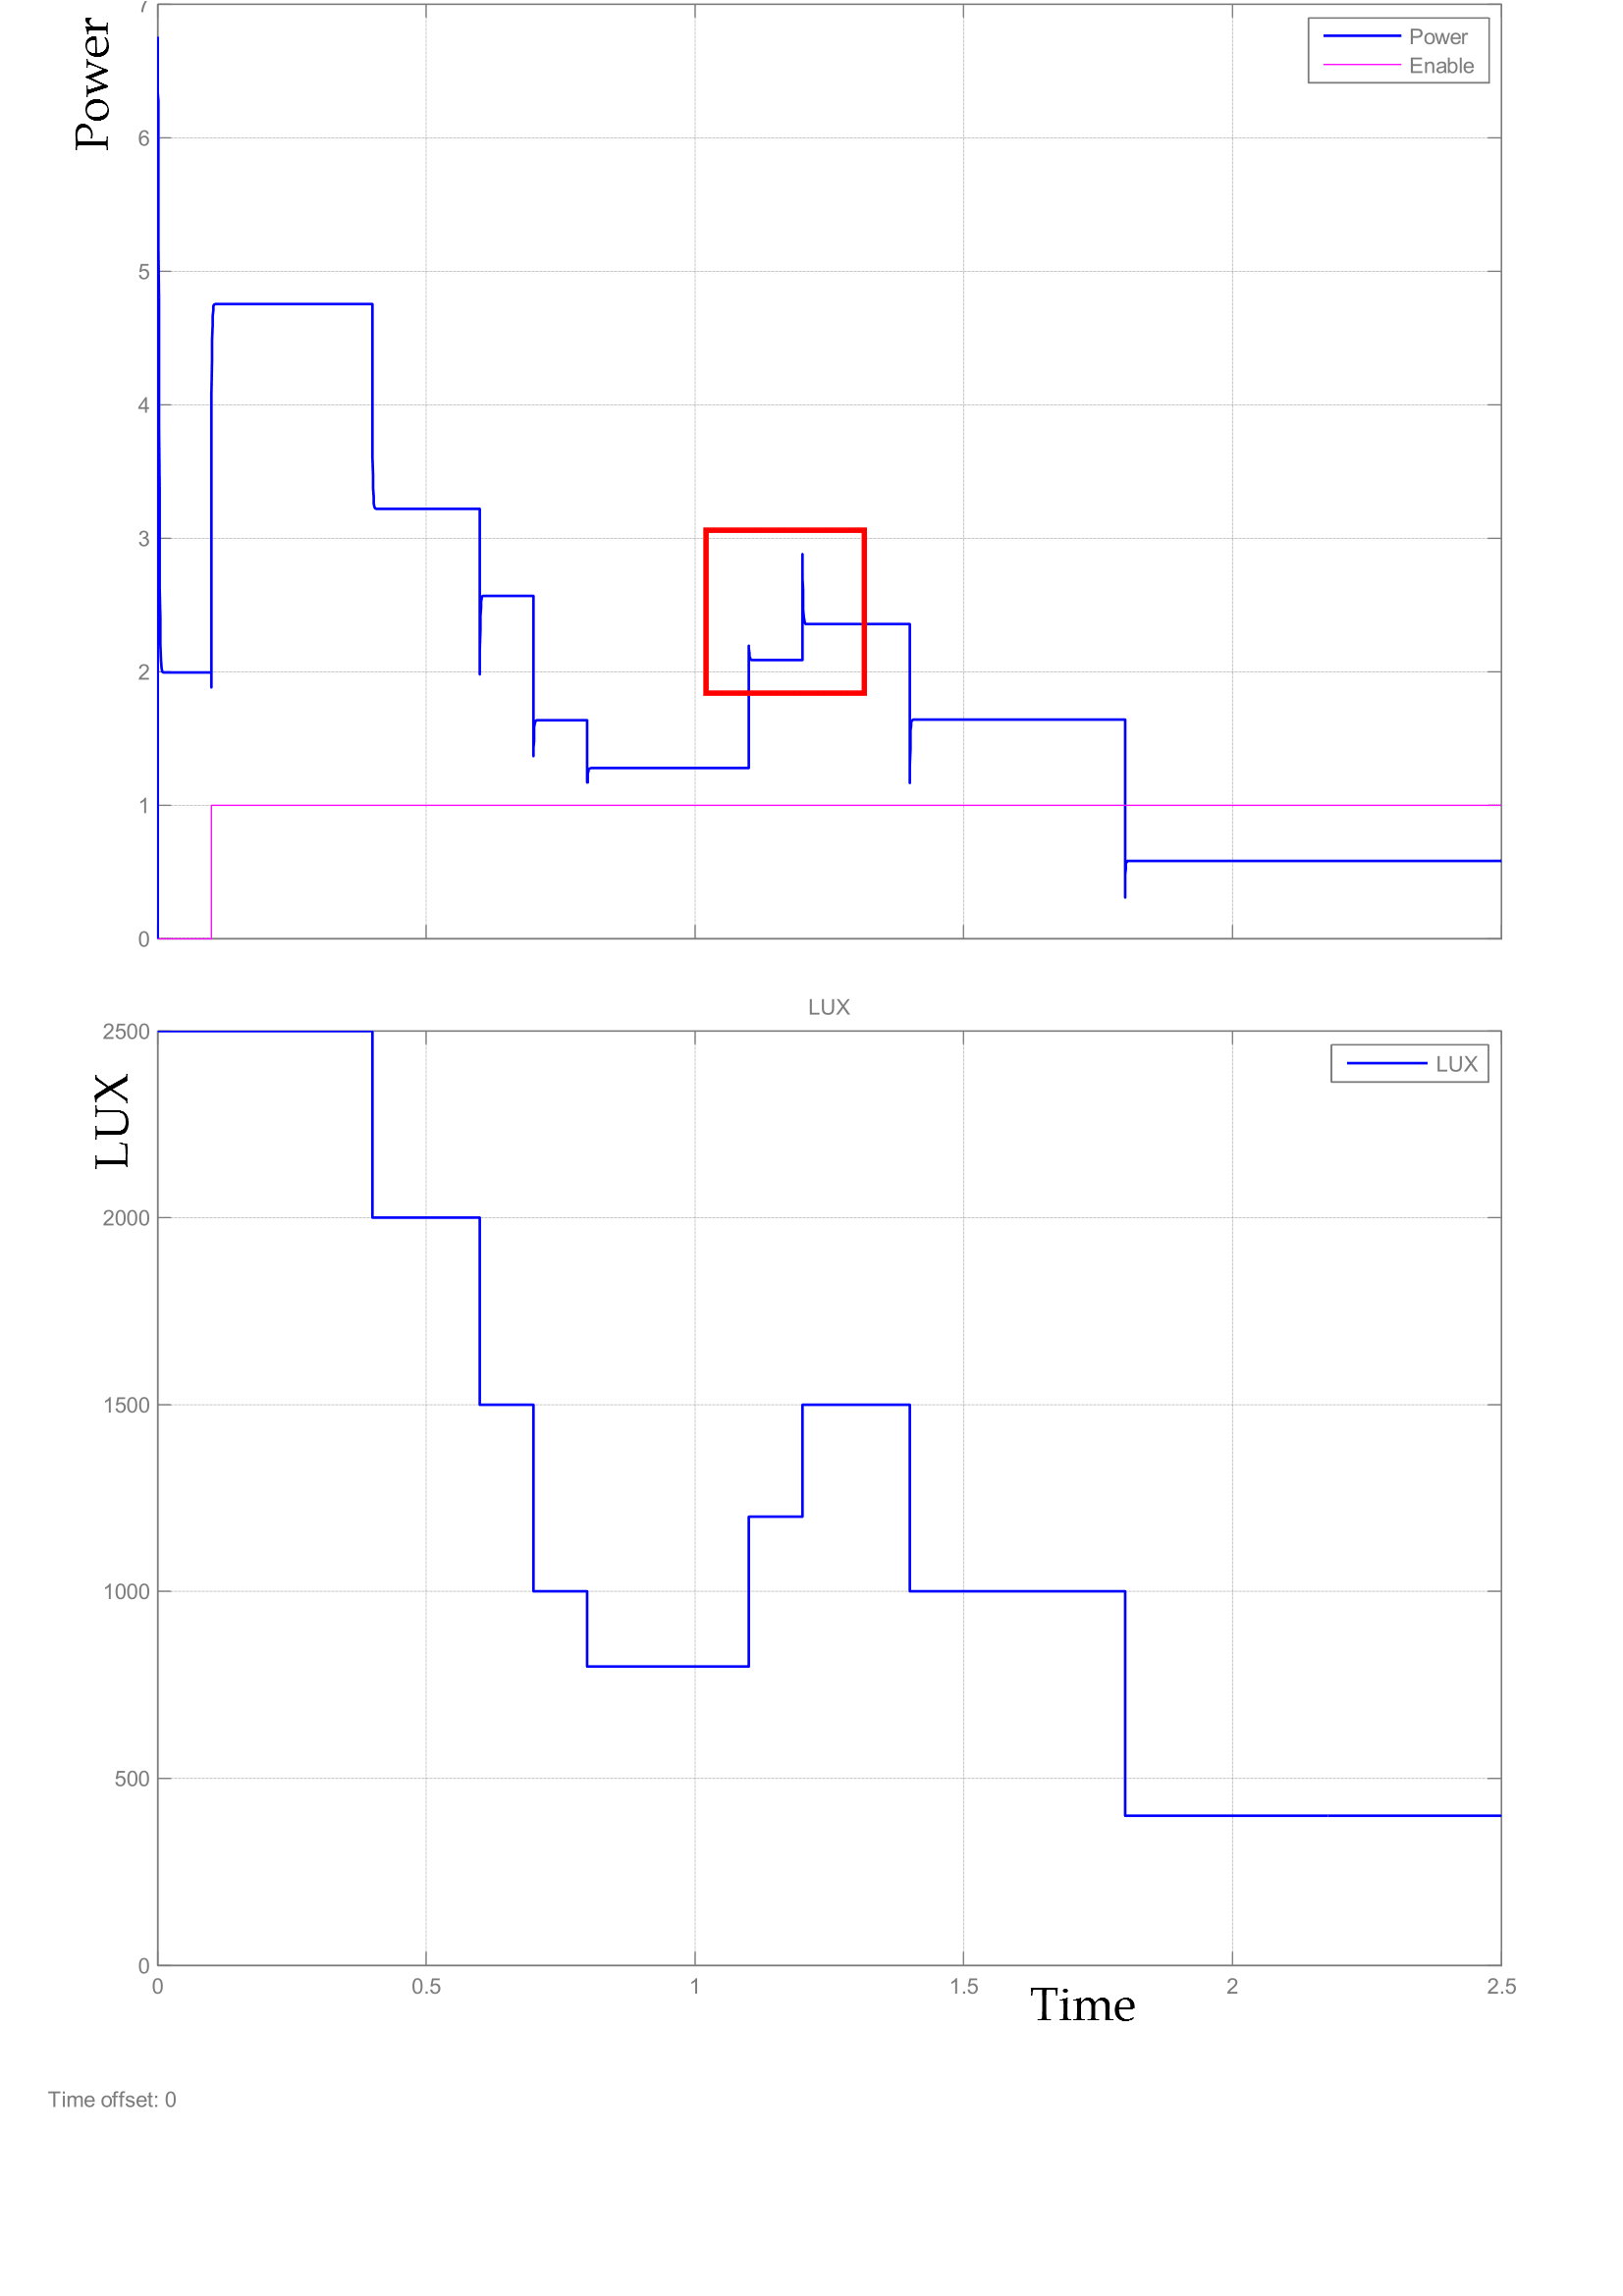
\includegraphics[width=\textwidth]{images/proposed_step_input}
  \caption{Proposed algorithm under rapidly varying light conditions with empty lookup tables }
  \label{fig:proposed_empty_lookup}
  \end{center}
  \end{figure}


 \begin{figure}[H]
  \begin{center}
  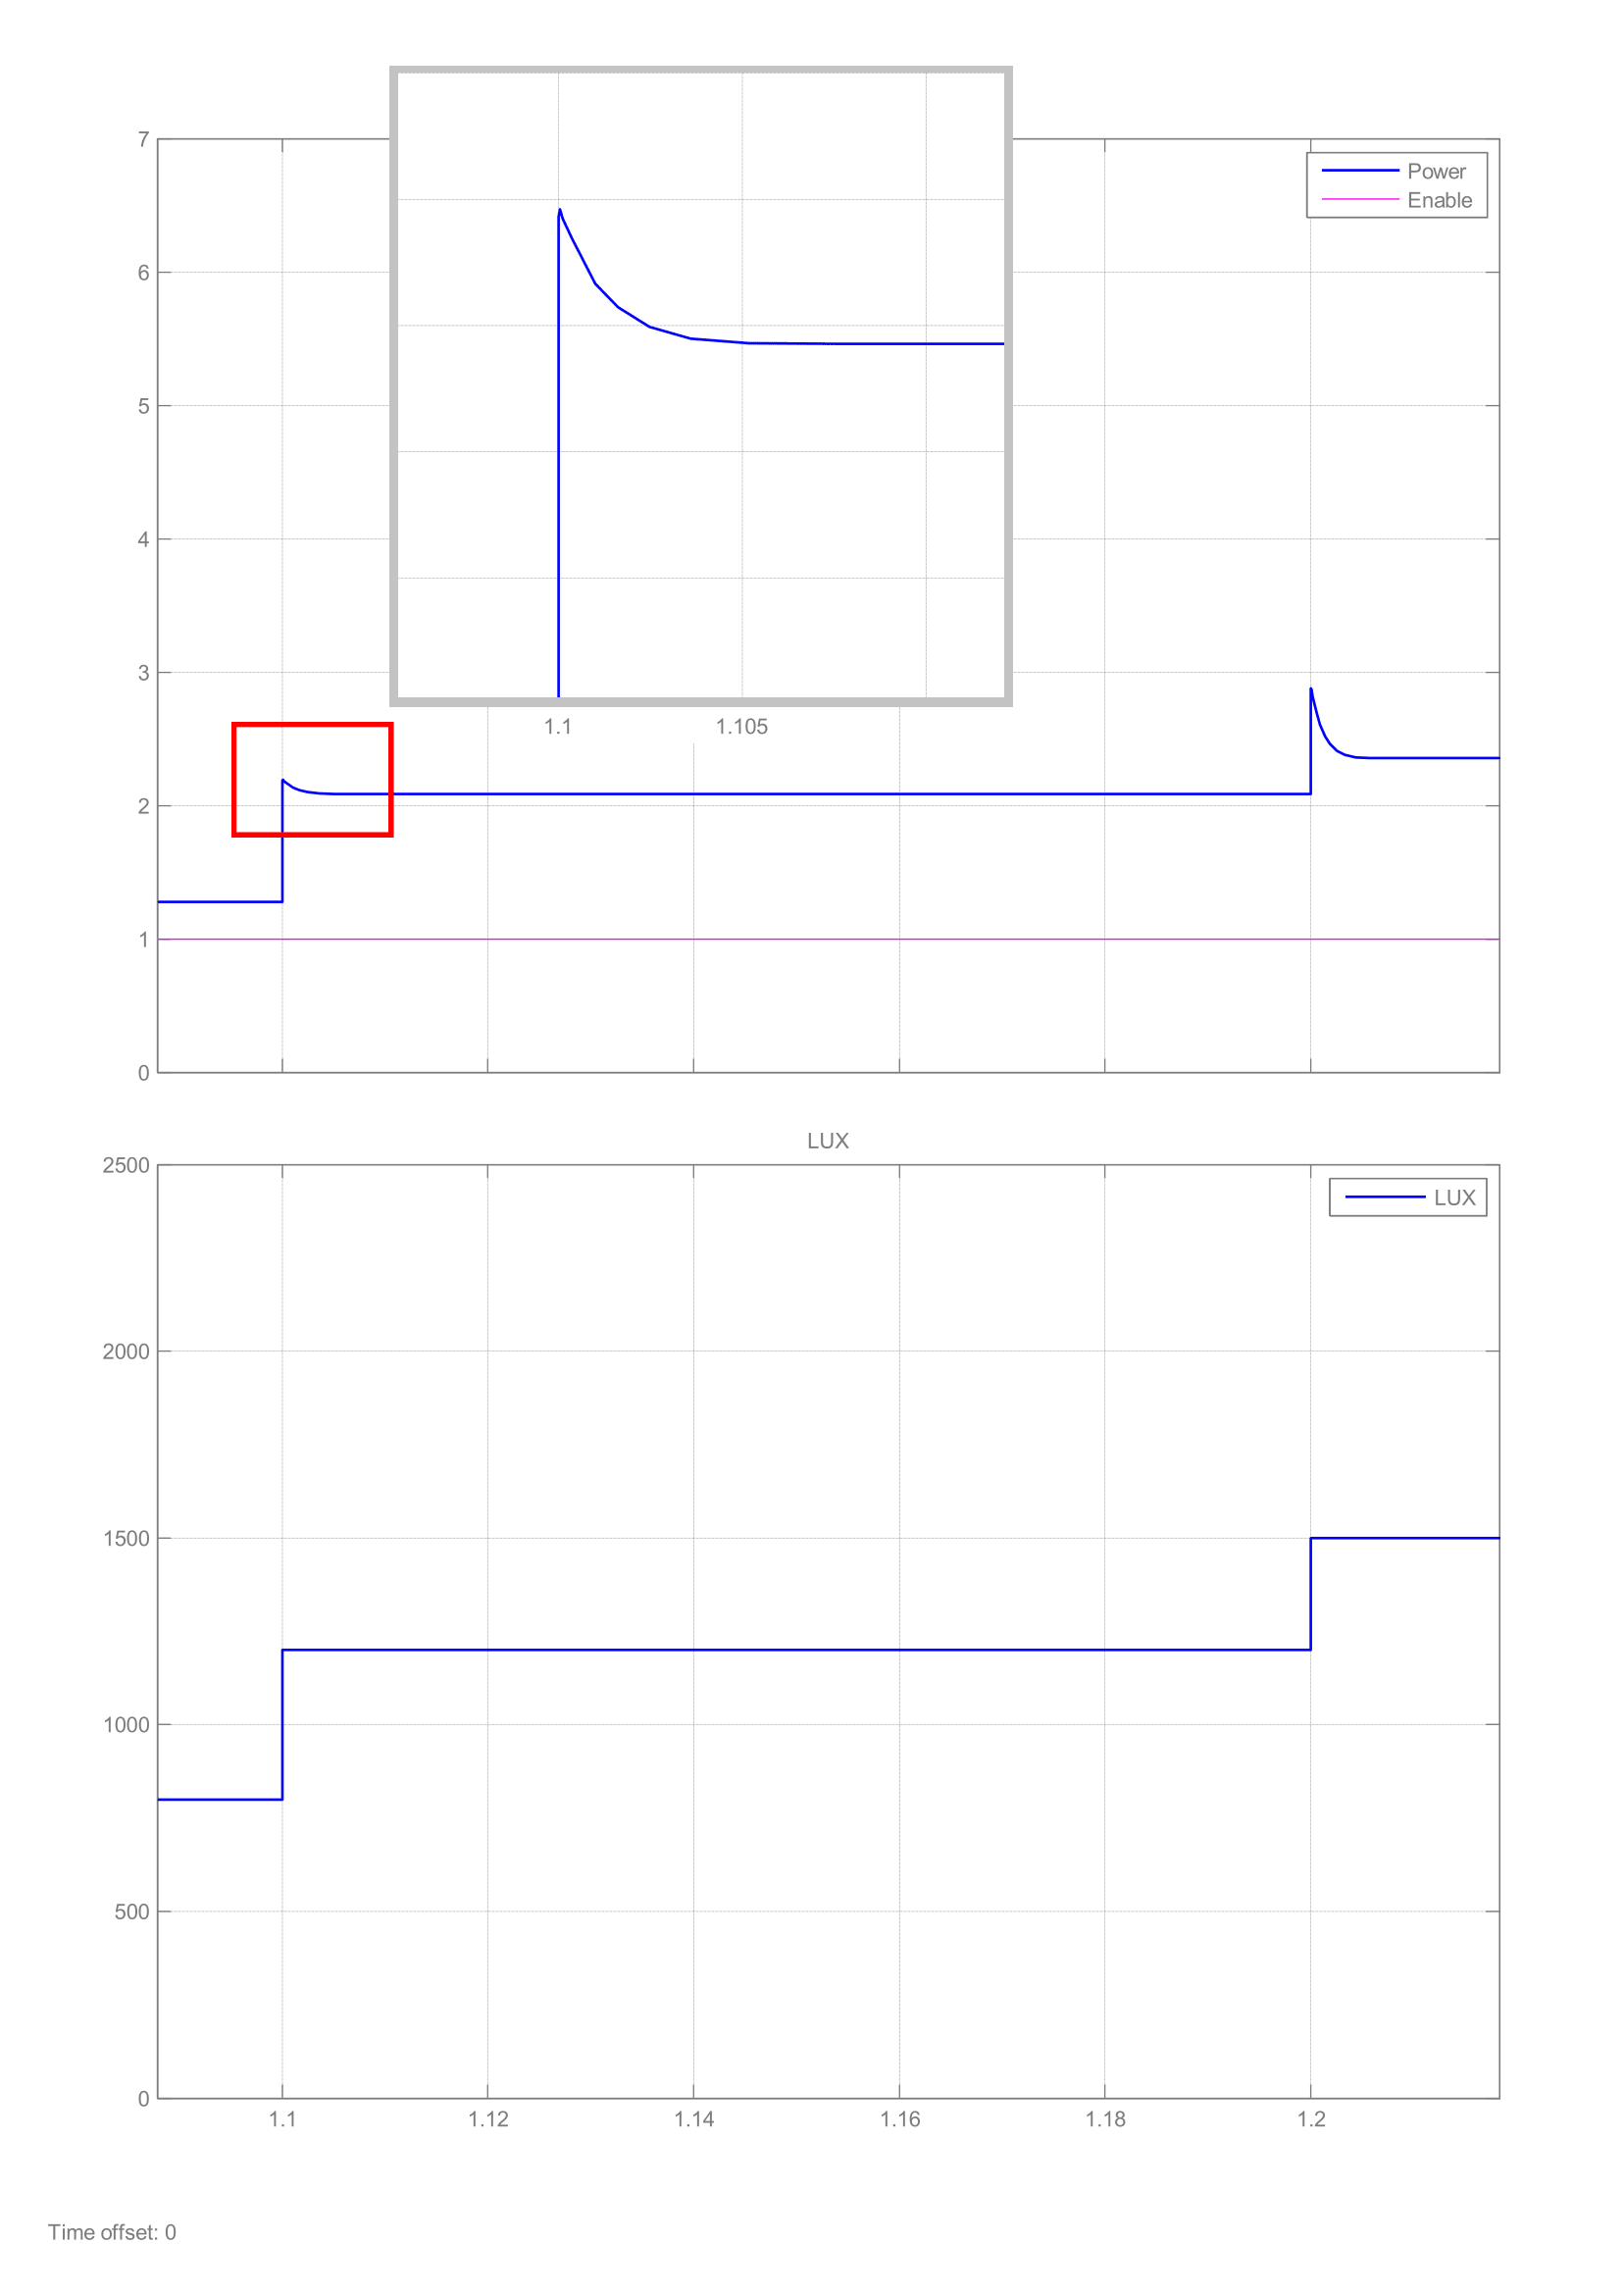
\includegraphics[width=\textwidth]{images/proposed_step_input_zoom-1(2)_pip}
  \caption{ expanded view of the graph in figure ~\ref{fig:proposed_empty_lookup}}
  \label{fig:fig:Zoom_proposed_empty_lookup}
  \end{center}
  \end{figure}

  
   \begin{figure}[H]
  	  \begin{center}
  		  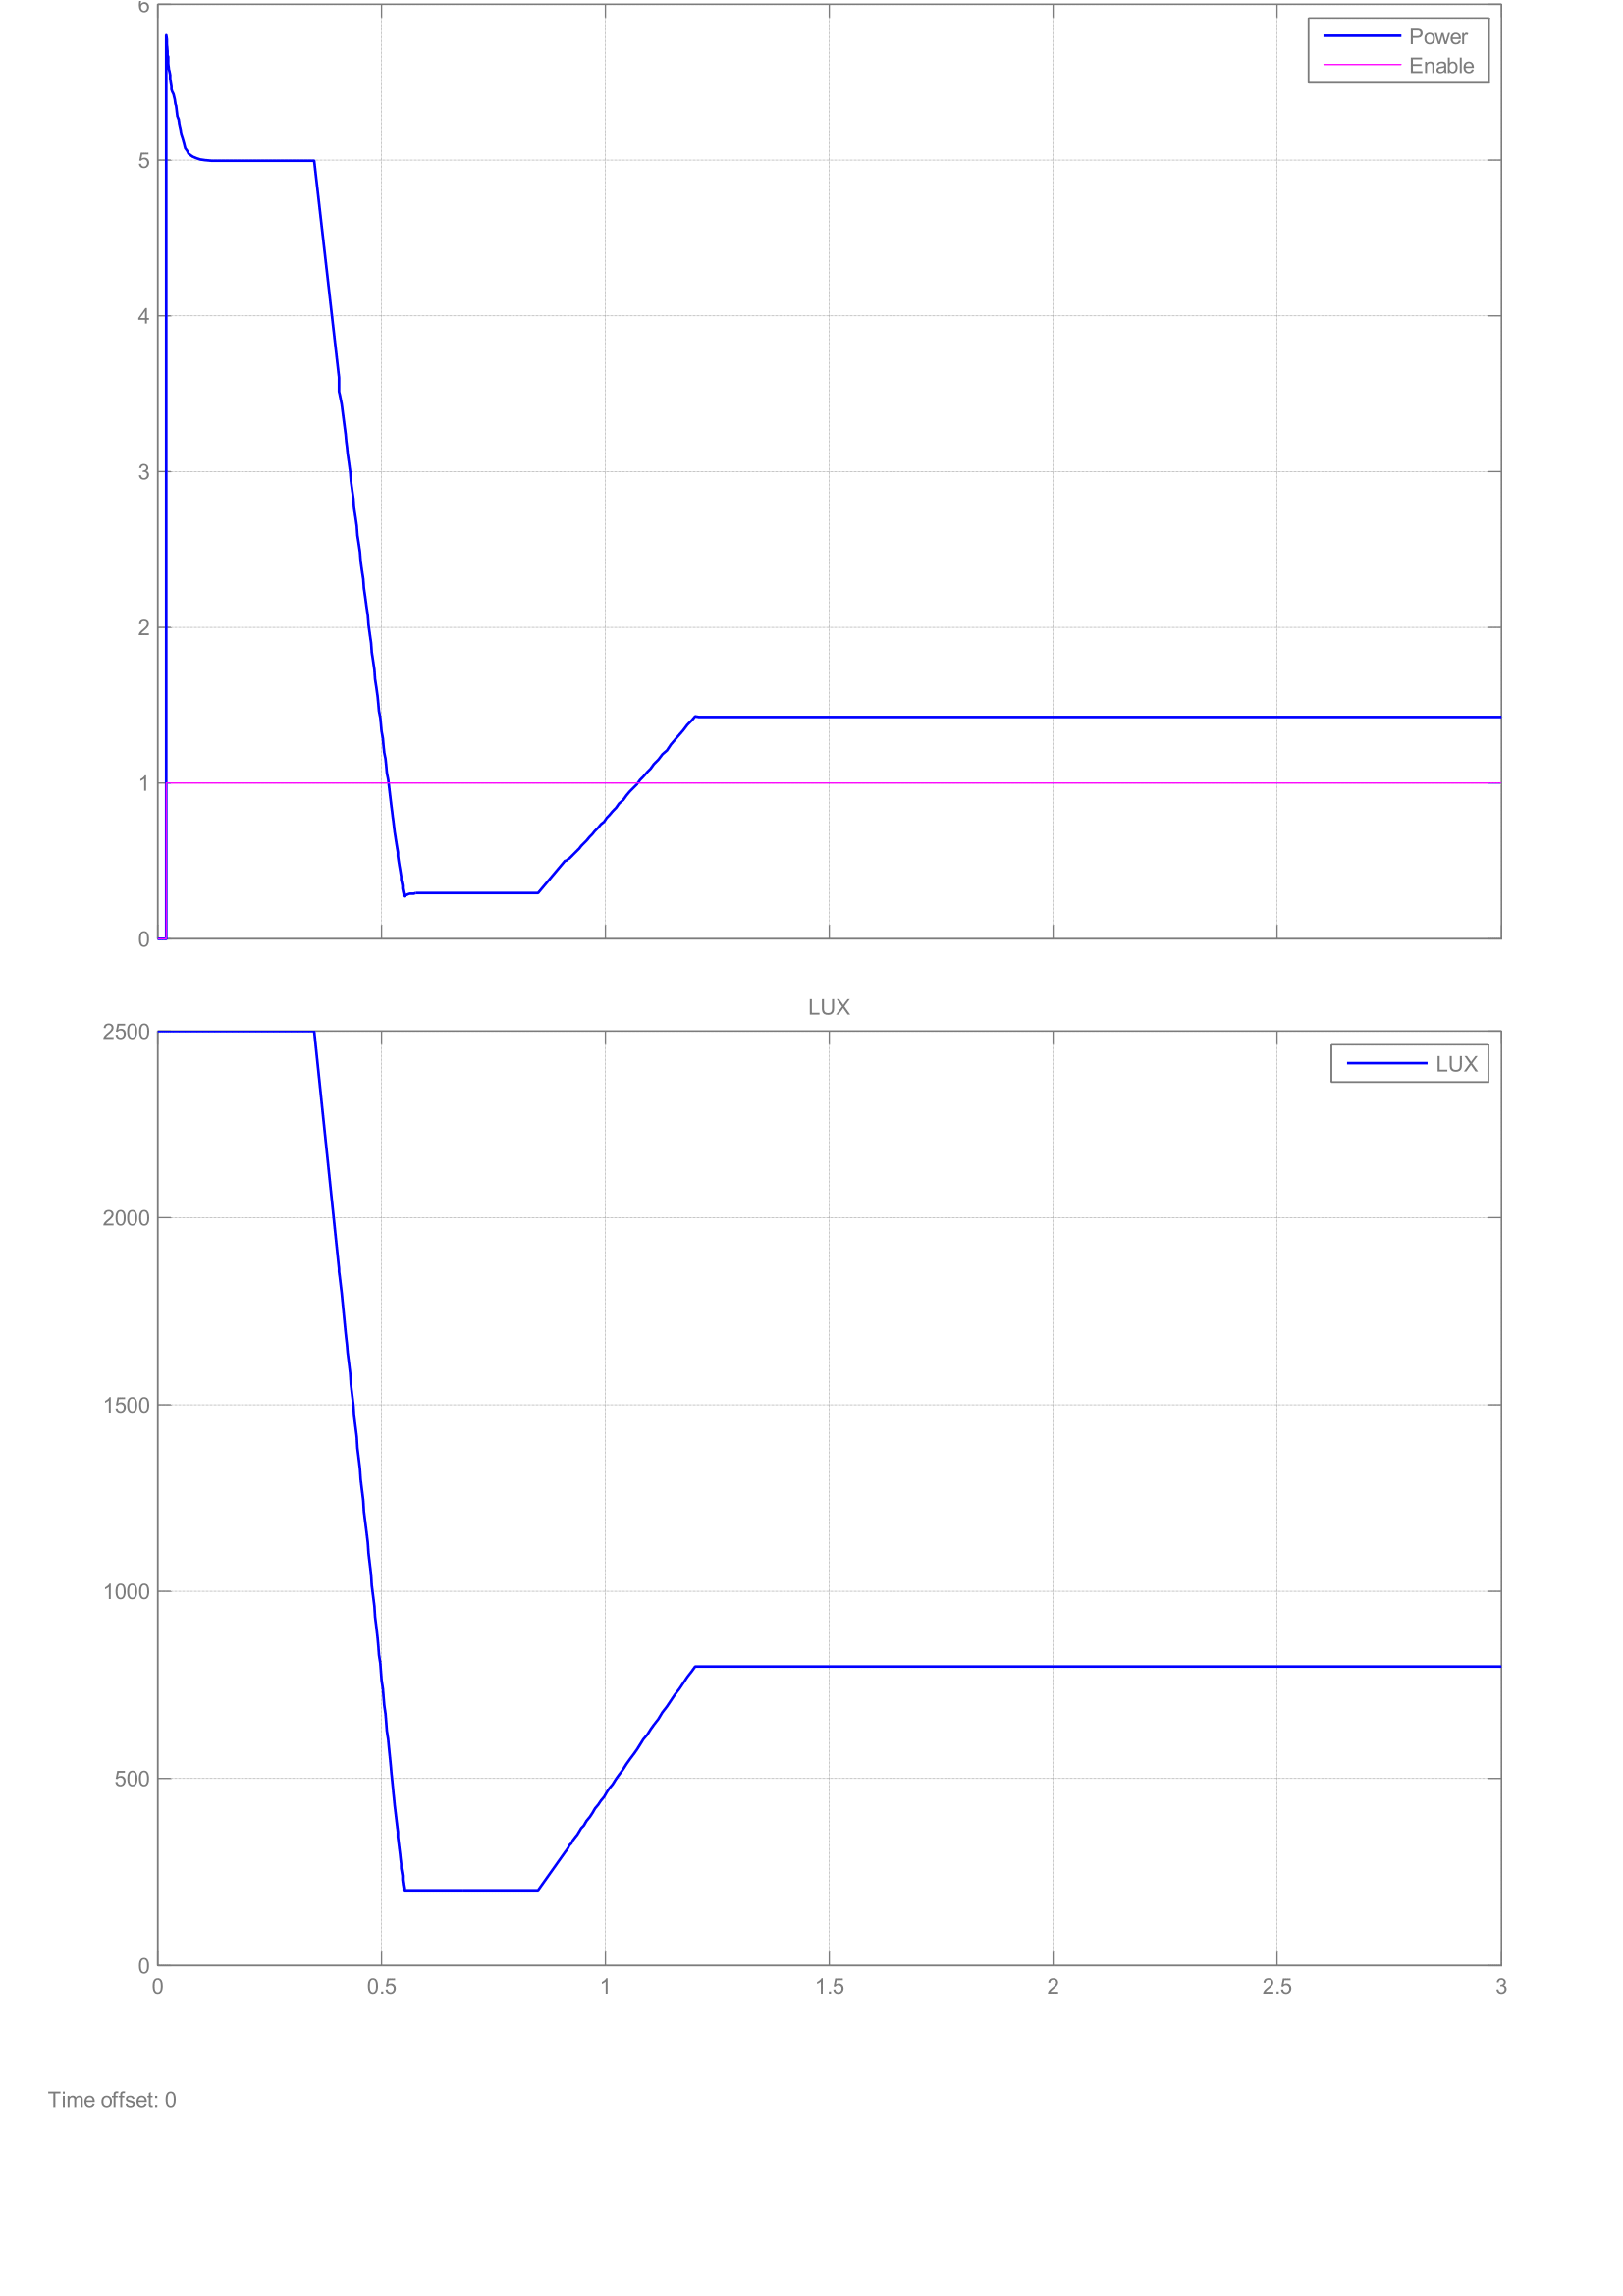
\includegraphics[width=\textwidth]{images/Proposed_algo-1}
  		  \caption{Proposed routine with full buffer, under similar light conditions as other algorithm}
  		  \label{fig:Frac_oc_result}
  	  \end{center}
    \end{figure}



